\documentclass[]{article}
\usepackage{lmodern}
\usepackage{graphicx}
\usepackage{amssymb,amsmath}
\usepackage{ifxetex,ifluatex}
\usepackage{fixltx2e} % provides \textsubscript
\ifnum 0\ifxetex 1\fi\ifluatex 1\fi=0 % if pdftex
  \usepackage[T1]{fontenc}
  \usepackage[utf8]{inputenc}
\else % if luatex or xelatex
  \ifxetex
    \usepackage{mathspec}
  \else
    \usepackage{fontspec}
  \fi
  \defaultfontfeatures{Ligatures=TeX,Scale=MatchLowercase}
\fi
\renewcommand{\figurename}{Rys.}
% use upquote if available, for straight quotes in verbatim environments
\IfFileExists{upquote.sty}{\usepackage{upquote}}{}
% use microtype if available
\IfFileExists{microtype.sty}{%
\usepackage[]{microtype}
\UseMicrotypeSet[protrusion]{basicmath} % disable protrusion for tt fonts
}{}
\PassOptionsToPackage{hyphens}{url} % url is loaded by hyperref
\usepackage[unicode=true]{hyperref}
\hypersetup{
            pdftitle={Generacja grafu i odnalezienie najkrótszej ścieżki pomiędzy węzłami: graph},
            pdfauthor={Ulyana Petrashevich, Inga Maziarz}
            pdfborder={0 0 0},
            breaklinks=true}
\urlstyle{same}  % don't use monospace font for urls
\IfFileExists{parskip.sty}{%
\usepackage{parskip}
}{% else
\setlength{\parindent}{0pt}
\setlength{\parskip}{6pt plus 2pt minus 1pt}
}
\setlength{\emergencystretch}{3em}  % prevent overfull lines
\providecommand{\tightlist}{%
  \setlength{\itemsep}{0pt}\setlength{\parskip}{0pt}}
\setcounter{secnumdepth}{0}
% Redefines (sub)paragraphs to behave more like sections
\ifx\paragraph\undefined\else
\let\oldparagraph\paragraph
\renewcommand{\paragraph}[1]{\oldparagraph{#1}\mbox{}}
\fi
\ifx\subparagraph\undefined\else
\let\oldsubparagraph\subparagraph
\renewcommand{\subparagraph}[1]{\oldsubparagraph{#1}\mbox{}}
\fi
\renewcommand{\contentsname}{Spis treści}
% set default figure placement to htbp
\makeatletter
\def\fps@figure{htbp}
\makeatother


\title{\texttt{Specyfikacja implementacyjna}\\Generacja grafu i odnalezienie najkrótszej ścieżki pomiędzy węzłami - \texttt{graph} - Java}
\author{Ulyana Petrashevich, Inga Maziarz}
\date{17.05.2022}

\usepackage{fancyhdr}
\usepackage{lastpage}
\pagestyle{fancy}
\fancypagestyle{plain}{}
\fancyhf{}
\rhead{Specyfikacja implementacyjna}
\lhead{Graph - Java}
\cfoot{Strona \thepage \hspace{1pt} z \pageref{LastPage}}

\begin{document}
\maketitle
\tableofcontents
\thispagestyle{empty}
\newpage
\section{Informacje ogólne}\label{header-n231}
Program \texttt{graph} został napisany w języku \texttt{Java} w środowisku programistycznym \texttt{IntelliJ IDEA}. Graficzny interfejs użytkownika został zrealizowany przy użyciu technologii \texttt{JavaFX}. Współpraca i wersjonowanie odbywa się w repozytorium zdalnym w serwisie \texttt{GitHub}.

Po uruchomieniu programu wyświela się okno o wymiarach 850 x 800 przedstawiające główny interfejs aplikacji. Cały interfejs programu jest przedstawiony w trybie graficznym. Argumenty określające parametry generowanego grafu są przekazywane przez użytkownika z klawiatury do konkretnych pól edycyjnych lub poprzez przycisk opcji (w przypadku wyboru spójności). Reszta pól to przyciski wywołujące akcje, tj. zapisywanie, wczytywanie, generowanie grafu itd. Po podjęciu akcji przez użytkownika wygenerowany lub wczytany graf wyświetli się na czarnym polu na środku ekranu. Działanie wyboru węzłów i rysowania ścieżek odbywają się na głównym oknie interfejsu. Przyciski \texttt{save graph}, \texttt{save path}, \texttt{read} inicjują pojawienie się nowych okien z opcjami wyboru plików do zapisu/wczytania. Nowe okna są również inicjowane w przypadku wystąpienia komunikatów z ostrzeżeniem/błędem oraz przy wyborze palety kolorów używanych do kolorowania grafu. Wszystkie z okien można zamknąć przyciskiem \texttt{"x"} lub po zatwierdzeniu zmian, powracając w ten sposób do głównego okna.

\section{Opis modułów, pakietów i narzędzi}\label{header-n233}
Przy tworzeniu programu zostały użyte nastąpujące dodatki:

\begin{itemize}
    \item Moduł javafx.controls
    
    Moduł zawiera sterowniki i kompozycję dla graficznego interfejsu JavaFX. 
    \item Pakiet java.awt
   
    Zawiera klasy dla zbudowania interfejsu użytkownika i stworzenia grafik.
    \item Pakiet java.util
   
    Zawiera podstawowe klasy (m.in Arrays, ArrayList, Date).
    \item Pakiet java.io
   
    Dostarcza obsługę operacji wejścia/wyjścia.
    \item Biblioteka JUnit 
    
    Służy do przeprowadzania testów jednostkowych.
    \item Narzędzie Maven 
    
    Umożliwia automatyzację procesu budowania aplikacji.
    
    
\end{itemize}

\section{Diagram klas}\label{header-n283}
\begin{figure}[h!]
\begin{center}
  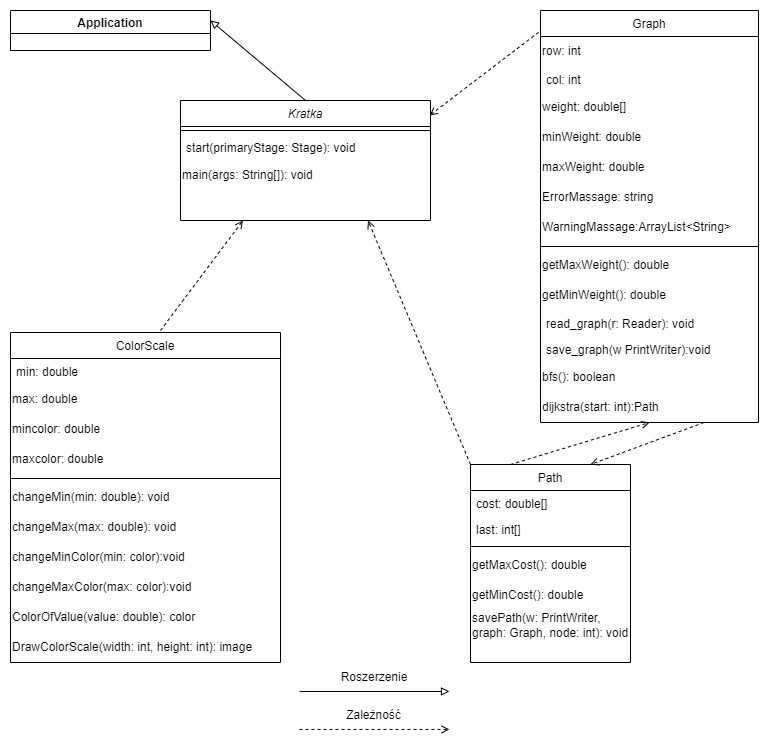
\includegraphics[scale=0.6]{diagram.png}
  \end{center}
  \caption{Diagram klas}
  \label{fig:graf}
\end{figure}

\section{Opis klas}\label{header-n233}
Klasy zawarte są w jednym z dwóch pakietów:

Pakiet "Kratka":
\begin{itemize}
    \item Kratka (dziedziczy po Application)
    
    Klasa odpowiada za wygląd i funkcjonowanie interfejsu graficznego. Zawiera funkcję main, uruchamiającą program. 
    
    Metody:
    \begin{itemize}
        \item start
        
        Metoda zastępuję metodę start, zdefiniowaną w klasie Application. W metodzie są zdefiniowane właściwości okna "Kratka", dodane etykiety, pola tekstowe, pole wyboru, przyciski z ustalonymi działaniami. 
        \item main
        
        Metoda odpowiada za uruchomienie aplikacji.
        
    \end{itemize}
    \item ColorScale
    
    Klasa odpowiada za zdefiniowanie i narysowanie skali kolorów.
    
    Metody:
    \begin{itemize}
    \item void changeMin(double min)
    
    Ustawia min jako wartość minimalną na skali. 
    \item void changeMax(double max)
    
    Ustawia max jako wartość maksymalną na skali.
    
    \item void changeMinColor(Color min)
    
    Metoda pozwala zmienić kolor wartości minimalnej na wybrany.
    \item void changeMaxColor(Color max)
    
    Metoda pozwala zmienić kolor wartości maksymalnej na wybrany.
    \item color ColorOfValue(double value)
    
    Zwraca kolor, odpowiadający wartości value zgodnie ze skalą.
    \item image DrawColorScale(int width, int height)
    
    Tworzy i zwraca rysunek skali kolorów o szerokości width i wysokości height. 
    \end{itemize}
\end{itemize}

Pakiet "Graph":
\begin{itemize}
    \item Graph
    
    Klasa definiuje postać przechowywania grafu i zawiera działania na grafie.  Reprezentacją grafu w kodzie jest macierz sąsiedztwa.
    Metody:
    \begin{itemize}
        \item double getMaxWeight()
        
        Metoda zwraca największą wagę krawędzi w grafie.
        \item double getMinWeight()
        
        Metoda zwraca najmniejszą wagę krawędzi w grafie.
        \item void generateGraph(boolean connect)
        
        Metoda generuje krawędzie do grafu. Spójność jest określona przez flagę connect.
        \item void readGraph(Reader r)
        
        Metoda wykorzystuje plik otwarty w czytniku r, nadaje grafowi wczytane wartości liczb wierszy i kolumn i dodaje krawędzie.
        \item void saveGraph(PrintWriter w)
        
        Metoda zapisuje graf do pliku, otwartego w zapisywaczu w.
        \item boolean bfs()
        
        Metoda służy do zastosowania algorytmu przeszukiwania grafu wszerz, aby sprawdzić, czy graf jest spójny. Zwróci wartość false, jeżeli graf będzie niespójny, wartość true - spójny.
        
        Algorytm BFS krok po kroku:
        \begin{itemize}
            \item Zaczynamy od węzła początkowego. Zaznaczamy go jako odwiedzony i dodajemy do kolejki wszystkie węzły, z którymi jest powiązany, w kolejności od węzła z najmniejszym indeksem.
            \item Odwiedzamy następny węzeł w kolejce. Dodajemy do kolejki wszystkie węzły z nim powiązane i jeszcze nieodwiedzone.
            \item Powtarzamy poprzedni krok, aż kolejka będzie pusta. Jeżeli wszystkie węzły w grafie zostały odwiedzone, to można stwierdzić, że graf jest spójny.
        \end{itemize}
        \item Path dijkstra(int st)
        Metoda służy do odnajdywania kosztów dojścia od podanego wierzchołka st do wszystkich innych w grafie za pomocą algorytmu Dijkstry.
        
        Algorytm Dijkstry krok po kroku:
        \begin{itemize}
            \item Dla każdego węzła ustawiamy długość ścieżki na nieskończoność lub wartość, która do niej dąży; długości przy węźle początkowym nadajemy wartość 0. 
            \item Oznaczamy węzeł jako odwiedzony. Dla każdego węzła połączonego z początkowym, przypisujemy długość równą wadze krawędzi ich łączących.
            \item Z nieodwiedzonych węzłów znajdujemy węzeł o najmniejszej przepisanej długości. Oznaczamy go jako odwiedzony. Dla każdego węzła sąsiadującego z obecnym liczymy wartość „długość przy obecnym węźle + waga krawędzi łączącej”. Jeżeli znaleziona wartość jest mniejsza niż przypisana do sąsiadującego węzła, podmieniamy ją.
            \item Powtarzamy poprzedni krok, aż zostaną odwiedzone wszystkie węzły. Po zakończeniu każdy węzeł będzie miał przypisaną długość najkrótszej ścieżki od węzła początkowego. Samą ścieżkę możemy odtworzyć od końca, jeżeli przy każdym przypisaniu węzłowi nowej długości będziemy zapamiętywali numer poprzedniego węzła.
        \end{itemize}
    \end{itemize}
    \item Path
  
    Klasa przechowuje listę wyliczonych kosztów dojścia do wierzchołków i listę poprzedników.
        \begin{itemize}
        \item double getMaxCost()
        
        Metoda zwraca największy koszt dojścia ze wszystkich.
        \item double getMinCost()
        
        Metoda zwraca najmniejszy koszt dojścia ze wszystkich.
        \item void savePath(PrintWriter w, Graph graph, int node)
        
        Metoda zapisuje ścieżkę do wierzchołka node do pliku, otwartego w zapisywaczu w.
    \end{itemize}
\end{itemize}

\section{Obsługa zdarzeń}\label{header-n279}

\begin{itemize}
    \item Pole "Size"
    
    Pole będzie pobierało od użytkownika rozmiar grafu za pomocą getText().
    \item Pole "Edge weight range"
    
    Pole będzie pobierało od użytkownika zakres wartości wag krawędzi za pomocą getText().
    \item Przycisk opcji "Connectivity"
    
    Element Radio Box będzie pobierał wybraną opcję spójności grafu (jedną na raz) za pomocą ButtonGroup.getSelection().getActionCommand().
    \item Przycisk "Generate"
    
    Przycisk będzie uruchamiał wczytywanie wartości z pól "Size", "Edge weight range" i przycisku opcji "Connectivity" i uruchamiał generator grafu. Wartości te będą przekazywane do generatora w klasie Graph.
    \item Przycisk "Read"
    
    Przycisk uruchomi wyświetlanie okienka do wyboru pliku do wczytania grafu, uruchomi jego wczytanie do programu i narysowanie w interfejsie graficznym. Jedynym akceptowanym formatem pliku jest format tekstowy \texttt{*.txt} (niemożliwe jest wybranie pliku o innym formacie). Filtrowanie formatu odbywa się przy użyciu getExtensionFilters().addAll(). Sprawdzana będzie poprawność zawartości pliku, to znaczy jego zgodność z przyjętą konwencją zapisu grafu, która jest następująca:
    
    W pierwszej linii pliku podana jest liczba wierszy i kolumn grafu. Parametry do jednego węzła są definiowane poniżej w jednej linii. Numer węzła docelowego jest oddzielany od wagi spacją i znakiem \texttt{:}. Parametry dla jednego węzła są oddzielane dwiema spacjami.
    
    Przykładowy plik:
    \begin{verbatim}
2 3
	 1 :0.8864916775696521  2 :0.2187532451857941 
	 0 :0.2637754478952221  5 :0.5486221194511974
	 3 :0.5380334165340379
	 2 :0.5486221194511974  5 :0.25413610146892474
	 3 :0.31509645530519625  0 :0.40326574227480094
	 4 :0.44272335750313074
\end{verbatim}
    Jeżeli format będzie prawidłowy, wywołana zostanie metoda rysująca graf. W przypadku błędu pojawi się wyjątek i zostanie wyświetlony komunikat.
    
    \item Przycisk "Save graph"
    
    Przycisk wyświetli okienko do utworzenia pliku do zapisania obecnego grafu i uruchomi jego zapisywanie w formacie tekstowym \texttt{*.txt}. Konwencja zapisu grafu do pliku jest tożsama z przedstawioną powyżej (Przycisk Read).
    \item Przycisk "Save path"
    
    Przycisk wyświetli okienko do utworzenia pliku do zapisania wybranych ścieżek i uruchomi zapisywanie w formacie tekstowym \texttt{*.txt}. Przykładowa treść zapisywana do pliku wygląda następująco:
    
    \begin{verbatim}
    Najkrótsza ścieżka:
        0 -0.1635472537235685- 3 -0.6524342534143475- 5
    Długość ścieżki jest równa 0.815981507137916
        \end{verbatim}
    Do pliku zapisywane będą wszystkie ścieżki na rysunku grafu obecne w momencie zapisywania. 
    \item Przycisk "Clear"
    
    Przycisk usunie wszystkie wyznaczone ścieżki w grafie.
    \item Przycisk "Delete"
    
    Przycisk usunie rysunek grafu z interfejsu.
    \item Modify color range
    
    Przycisk zainicjuje wywołanie okna z wyborem zakresu kolorów używanych do rysowania ścieżek w grafie. Możliwy będzie wybór koloru oznaczającego wierzchołek o maksymalnym i minimalnym koszcie dojścia, krawędź o największej i najmniejszej wadze oraz kolor używany do rysowania ścieżki.
    \item Klikanie lewym klawiszem myszki na wierzchołek
    
    Kliknięcie na dany wierzchołek lewym przyciskiem myszy oznaczy go jako wierzchołek początkowy. Możliwe jest ponowne wybranie wierzchołka początkowego poprzez kliknięcie na inny wierzchołek. Dopóki nie zostanie wybrany wierzchołek końcowy, to nie rozpocznie się żadna akcja. 
    
    
    \item Klikanie prawym klawiszem myszki na wierzchołek
    
    Kliknięcie na dany wierzchołek prawym przyciskiem myszy oznaczy go jako wierzchołek końcowy. Wybranie wierzchołka końcowego musi nastąpić po uprzednim wybraniu wierzchołka początkowego (kolejność wyboru nie może być zmieniona). Jeśli uprzednio żaden wierzchołek nie został wybrany jako początkowy, to nie rozpocznie się żadna akcja. W przypadku, gdy wierzchołki zostaną wybrane prawidłowo, uruchomiony zostanie algorytm BFS do sprawdzenia spójności grafu. Po jego pomyślnym zakończeniu zostanie uruchomiony algorytm Dijkstry. Nastąpi przypisanie kolorów do każdego z wierzchołków z zakresu Node Color Range. Wartości kolorów odwzorowują koszty dojścia do każdego z wierzchołków od wierzchołka początkowego. Najkrótsza ścieżka między wierzchołkiem końcowym a początkowym zostanie narysowana i pokolorowana (w przypadku domyślnym) na biało.

\end{itemize}

\section{Budowa GUI}\label{header-n279}

\begin{figure}[h!]
\begin{center}
  \includegraphics[scale=0.6]{graf.png}
  \end{center}
  \caption{Projekt głównego okna interfejsu}
  \label{fig:graf}
\end{figure}

\section{Testowanie}\label{header-n281}
Testy są generowane przy pomocy biblioteki JUnit umożliwiającej przeprowadzanie testów jednostkowych. Testy przechowywane są w folderze \texttt{src/test/java}. Testowana jest większość obecnych w kodzie metod, a rodzaj asercji jest zależny od typu zwracanego przez metodę.

\begin{itemize}
    \item assertTrue();
    
    używane do metod zwracających typ boolean, np. \texttt{boolean bfs()}. Przykładowo, algorytm bfs jest testowany na znanych grafach (zarówno spójnych i niespójnych); dla spójnego powinien zwracać wartość true, a dla niespójnego - false.
    
    \item assertEquals();
    
    używane do metod zwracających typ double, np. \texttt{double getMaxCost(), double getMaxWeight()}. W tych testach korzystamy ze znanych wartości długości wag i kosztów w danym grafie i przyrównujemy wartości zwrócone przez metody z oczekiwanymi.
    
    \item assertArrayEquals();
    
    używane do algorytmu Dijkstry w celu sprawdzenia poprawności wyznaczania najkrótszej ścieżki oraz jej przebiegu.
    
    
    \item assertThrows();
    
    używane do metod zwracających typ void, np. \texttt{void readGraph(Reader r), void generateGraph(boolean connect)}. Testy mają na celu wyłapanie błędów dotyczących nieprawidłowo podanych parametrów przy tworzeniu obiektu grafu, niezgodności formatu wczytywanego pliku.
\end{itemize}

Przykładowe testy jednostkowe:

Poniższy test ma na celu sprawdzenie, czy metoda \texttt{boolean bfs()} zwróci wartość \texttt{true} w przypadku podania grafu spójnego.

\begin{verbatim}
@Test
public void ConnectedGraphTrue1(){
    
    Graph graph = new Graph(2, 3, {0.00, 1.00, 0.00, 4.00, 0.00,
    0.00, 1.00, 0.00, 3.00, 0.00, 0.00, 0.00, 0.00, 3.00, 0.00,
    0.00, 0.00, 7.00, 4.00, 0.00, 0.00, 0.00, 0.00, 0.00, 0.00,
    0.00, 0.00, 0.00, 0.00, 2.00, 0.00, 0.00, 7.00, 0.00, 2.00, 0.00}
        
    Assert.assertTrue(graph.bfs());
    }
\end{verbatim}

Poniższy test ma na celu sprawdzenie, czy metoda \texttt{double getMaxWeight()} zwróci największą długość wagi w grafie.

\begin{verbatim}
@Test
public void MaxWeight7(){
    
    Graph graph = new Graph(2, 3, {0.00, 1.00, 0.00, 4.00, 0.00,
    0.00, 1.00, 0.00, 3.00, 0.00, 0.00, 0.00, 0.00, 3.00, 0.00,
    0.00, 0.00, 7.00, 4.00, 0.00, 0.00, 0.00, 0.00, 0.00, 0.00,
    0.00, 0.00, 0.00, 0.00, 2.00, 0.00, 0.00, 7.00, 0.00, 2.00, 0.00}
        
    Assert.assertEquals(7, graph.getMaxWeight());
    }
\end{verbatim}

Poniższy test ma na celu sprawdzenie poprawności generowania spójnego grafu przez metodę \texttt{void generateGraph(boolean connect)}. Będzie także przeprowadzony test na generowanie grafu niespójnego z podobnym algorytmem.
\begin{verbatim}
    @Test
    void CheckGenerationOfConnectedGraph() {
        graph = new Graph(3, 2);
        graph.generateGraph(true);
        assertTrue(graph.bfs());
    }
\end{verbatim}

Poniższy test ma na celu sprawdzenie poprawności metod zapisywania i odczytywania pliku \texttt{void saveGraph(PrintWriter w)} i \texttt{void readGraph(Reader r)}. 
\begin{verbatim}
    @Test
    void CheckReadingAndSaving(){
        graph = new Graph(3,2);
        graph.generateGraph(true);
        File write;
        write = new File("filename.txt");
        try {
            PrintWriter w = new PrintWriter (write);
            graph.saveGraph(w);
        } catch (FileNotFoundException e) {
            throw new RuntimeException(e);
        }
        Graph graph1 = new Graph();
        Reader r;
        try {
            r = new FileReader(write);
            graph1.readGraph(r);
        } catch (FileNotFoundException e) {
            throw new RuntimeException(e);
        }
        assertEquals(graph.row, graph1.row);
        assertEquals(graph.col, graph1.col);
        assertArrayEquals(graph.weights, graph1.weights);
    }
\end{verbatim}
Reszta testowania odbywa się w środowisku graficznym, poprzez korzystanie z opcji interfejsu i sprawdzanie, czy wyniki działania są zgodne z oczekiwanymi.
\end{document}
